\section{Know Thyself}

\begin{quote}
{\em Know thyself.} --- inscribed on the Temple of Apollo at Delphi
\end{quote}

We cannot follow the advice of Newell before we name the strengths.
Self-report names them badly.
Thus, before we read the literature, we first make machines read us.
The record of our own papers shows the team.

Our instrument is the repertory grid of Kelly~\cite{kelly55}.
Kelly said that people understand a domain through distinctions with
two poles.
He called these distinctions constructs.
Triads make the grid.
Show three team members, then ask which one stands apart, and on which
dimension.
Each answer gives one construct.
Stop when no new dimension appears, then rate each person on each
construct.

Data collection took minutes.
For six authors of this paper, an agent got the five most-cited papers
of all time, and the five most-cited papers of the last five years.
The agent scanned about 1,200 paper records.
It coded the papers against the ICSE'27 research areas.
Then it was the interviewee in the triads.
We merged the constructs that agreed at more than
90\%.\footnote{Caveats: there was one rater (the agent); citation
counts were the only measure of strength; two young authors have few
papers.}
Figure~\ref{fig:focus} shows the result after FOCUS sorting.
Rows and columns move so that similar neighbors touch.
Poles turn so that neighbors align.
Trees join only adjacent clusters.

\begin{figure}[t]
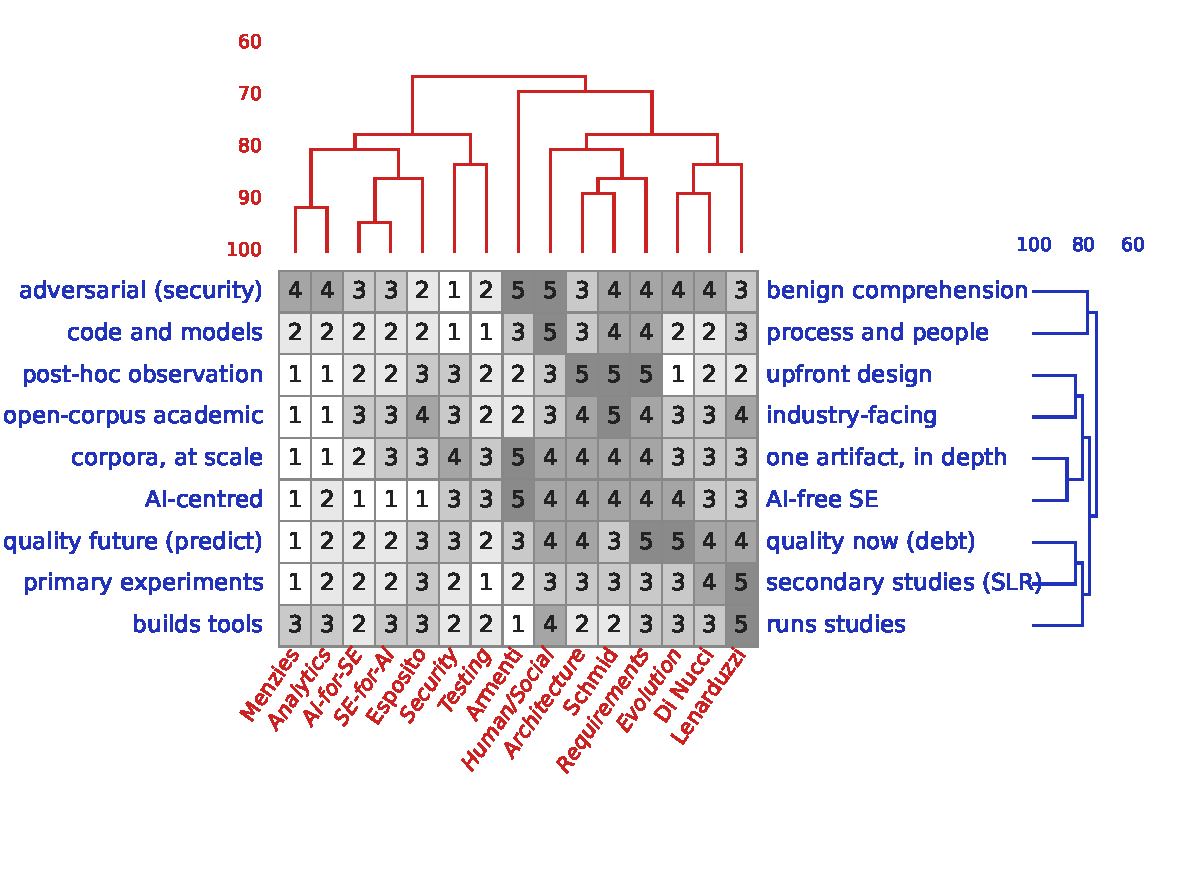
\includegraphics[width=\linewidth]{fig/focus_grid}
\caption{The repertory grid of six authors (upright columns) plus
the nine ICSE'27 areas as reference elements (italic columns; see
\S\ref{sec:map}).
Grey cells score each column from the left pole (1) to the right pole
(5) of each construct.
Trees join neighbors by percentage match.
To make this figure again, use {\em make focus}.}
\label{fig:focus}
\end{figure}

The grid gives three readings.
First, near-synonyms: construct rows that merge early name one
dimension twice.
In this team, corpus-scale work and AI-centred work travel together,
and primary experiments travel with future prediction.
Second, birds of a feather: Lenarduzzi and Di Nucci match at about
90\%.
They are the quality-and-evolution core of the team.
Third, complements: Schmid and Armenti sit far from that core.
Upfront design and single-artifact comprehension are rare skills here,
and one member holds each.

Thus, the grid is two things at one time.
It is a division of labor, and it is a price list of the blind spots
of the team.
We computed it before we read one outside paper.

\begin{pause}{the grid}
Ask: are the construct poles the distinctions that you would make?
Are any ratings unfair to a colleague?
Must we add or remove a person or a construct?
Are five top-cited papers for each author the correct evidence
base?\\[0.2em] To change the outcome: edit the {\ttfamily CONSTRUCTS}
table (or {\ttfamily ELEMENTS}) in {\ttfamily focus.py}, then do
{\ttfamily make focus}; the trees, the pairs of \S\ref{sec:map}, and
the topic arithmetic all follow from that one table.
\end{pause}
